\section{Description of the Algorithm}

Early detection of melanoma greatly increases the chances of successful treatment. A biopsy can be performed in order to gain a definitive diagnosis. However, biopsies are invasive, painful and take time. There are also visual markers Dermatologists look for in order to make a risk assessment. The ABCD Rule, also known as Stokes or TDS Calculation, looks for 4 sets of features. Based on the features the Total Dermoscopy Score (TDS) is calculated.

The 4 sets of features are Asymmetry (A), Border Irregularity (B), Color (C) and Differential Structure or Diameter (D).

Asymmetry can have a value of 0, 1 or 2 depending on the symmetry of the lesion. Where 0 is symmetric and 2 is asymmetric. A value of 1 indicates at least one axis was found across which symmetry exists. The Border score is an integer value from 0 to 8 indicating the presence of border irregularities in 8 regions. Color is an integer value from 1 to 6 indicating the presence of one to six specific colors. Similarly, the value for D indicates the presence of one to five distinct structures or textures. Alternatively, in some literature\cite{Siddiq_2015} D is defined as Diameter, where a diameter greater than 6mm results in a value of 5, otherwise 1.

The final TDS Score is the weighted sum of the ABCD Values and is in the range 1.0 to 8.9.

\begin{equation}
TDS = A * 1.3 + B * 0.1 + C * 0.5 + D * 0.5
\end{equation}

A diagnosis can be made based on the TDS Score according to the following table:

\begin{table}[H]
\centering
\small
    \begin{tabular}{ | l | p{3.5cm} | l | p{3.5cm} |}
    \hline
    Evaluation & TDS Score \\ \hline
    Benign & \textless  4.75  \\ \hline
    Suspicious & 4.75 to 5.45  \\ \hline
    Malignant & \textgreater  5.45  \\ \hline

    \end{tabular}

    \caption{TDS Evaluation\cite{Weigert_2012}}
    \label{fig:tds_eval}

\end{table}


\section{Automatic Calculation of ABCD Values}

The ABCD Rule is used by Dermatologists to differentiate benign from malignant melanocytic tumors. Because it is a clearly defined rule based on easily recognizable visual features it is easy to apply. Clinicians with limited dermoscopy experience achieve better results using the ABCD rule than other methods \cite{Weigert_2012}. The following sections detail methods to automate the calculation of the ABCD scores.

\subsection{Asymmetry}

The "Center of mass" method of measuring asymmetry is relatively easy to calculate and is more accurate compared to other complex algorithms \cite{Premaladha_2014}.

This algorithm begins by calculating an array of radii from the lesion's center of mass to border for each of 360 degrees. The coordinates for the center of mass are calculated from the sum of all x and y coordinates of pixels within the lesion's border each divided by the sum of pixels.

For each of the 360 radii $r_i$ a score is calculated by comparing the lengths of pairs of radii that are symmetric across $r_i$. If the lengths of the pair of symmetric radii have a difference of less than 10\% then a point is given. The sum of points is the $SFA_i$ (Score For Axis) for $r_i$.

\begin{figure}[H]
    \centering
    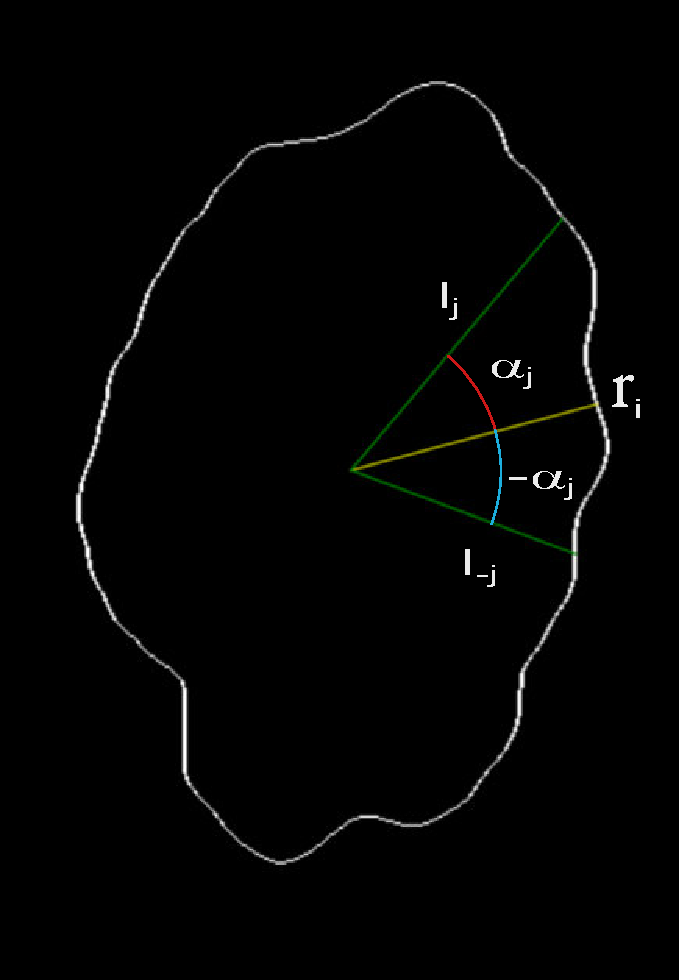
\includegraphics[height=6cm,keepaspectratio]{assets/assymertry/asymmetry_01.pdf}
    \caption{Calculate SFA for $r_i$}
    \label{fig:sfa}
\end{figure}


 The radius with the heighest SFA score is defined as the major axis of symmetry. The SFA of the major axis as well as the perpendicular are stored. The Asymmetry score is evaluated as follows:


\begin{table}[H]
\centering
\small
    \begin{tabular}{ | l | p{3.5cm} | l | p{3.5cm} |}
    \hline
    SFA Results & Description & Asymmetry Score \\ \hline
    \specialcell[t]{major axis $\geq$ 140 \\ minor axis $\geq$ 140} & Symmetric across both axis & 0  \\ \hline
    \specialcell[t]{major axis $\geq$ 140 \\ minor axis $\textless$ 140} & Symmetric across one axis & 1  \\ \hline
    \specialcell[t]{major axis \textless 140 \\ minor axis \textless 140} & Asymmetric & 2  \\ \hline


    \end{tabular}

    \caption{TDS Evaluation\cite{Weigert_2012}}
    \label{fig:tds_eval}

\end{table}


\subsection{Border}

\subsection{Color}

\subsection{Differential}

\section{Two Examples}
\subsection{Postitiv Example}

\subsection{False Example}

ABCD Values were calculated but classification result was false.

\section{Results of Algorithm}

Performance Evaluation

Chapters 11.1, 11.2, maybe 11.3